\section{Neural Networks} \label{ch:neural_networks}

As already mentioned, the name Neural Network has become widely accepted, although it is neither neural nor a network. % TODO citation needed (chollet)
They are used to create more complex mappings than the previous models were able to do.
In the following we will discuss what the motivation behind this concept is and how networks are trained.

\subsection{Deep learning} \label{ch:deep_learning}

Although the universal approximation theorem shows that all continuous functions can be described with only one layer, in practice it is much more reasonable to add several layers to our model to keep the required resources low.
Rolnick and Tegmark \cite{Rolnick2017} show that in single-layer models the number of neurons grows exponentially with the number of variables of the input, whereas multi-layer neural networks grow only linearly.

% TODO add some clues for notation
\begin{figure}
    \centering
    \caption[Neural Network]{ A neural network with three input nodes, two hidden layers with five nodes each and an output layer with three nodes. The bias is added to each layer by prepending a node with value one. Every node is, like the previous example calculated by the sum of the product of the previous layer and their respective weight.  }
    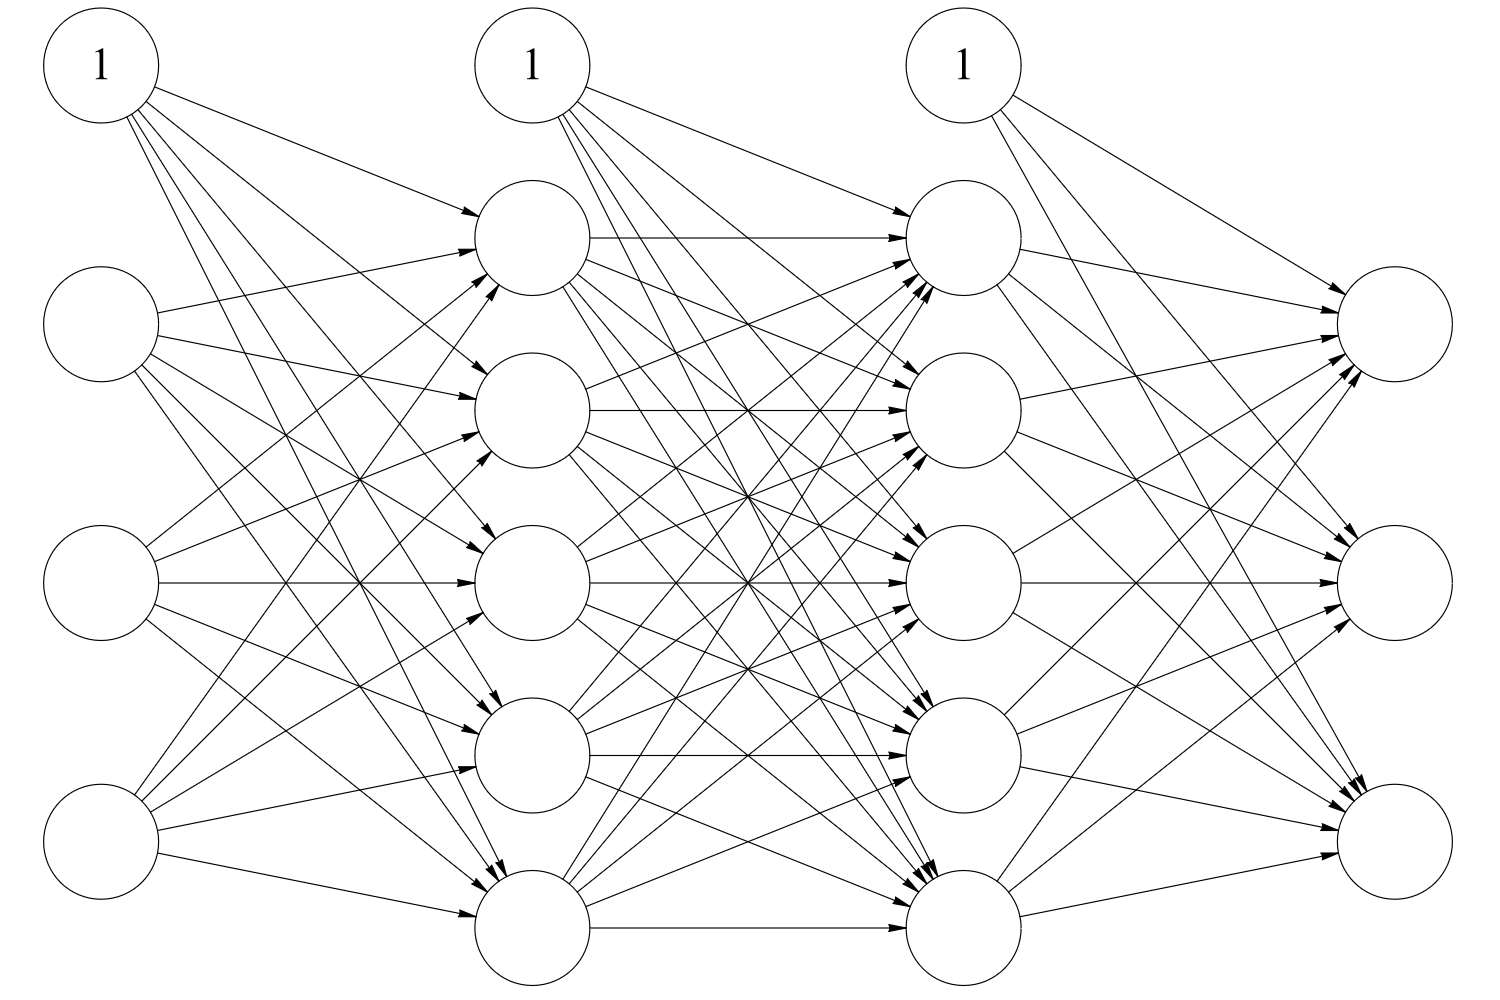
\includegraphics[width=0.6\textwidth]{images/2_nn_with_bias.png}
    \label{fig:nn}
\end{figure}

Each node in figure~\ref{fig:nn} can be addressed using the notation $z^l_i$.
$l$ is the number of the layer in which the node is located and $i$ is the index of the node.
Each weight $\theta^l_{i, j}$ can also be addressed; $l$ is the layer to which the weight refers, $i$ is the index of the node, which is multiplied by the weight to influence the value of the node in the layer $l$ with the index $j$.
So we can describe each node as the result of the following equation\footnote{In literature the bias is often added separately.
According to the convention of prefixing the input vector $x$ with a 1, it is always included as index 0 of each layer.
Please note that, mathematically this is the same.}:

\begin{equation}
    z^l_j = \sum^n_{i=0}z^{l-1}_i\theta^l_{i, j}
    \label{eq:node_value}
\end{equation}

$n$ is the number of nodes in the respective layer. Equation~\eqref{eq:node_value} can be vectorized to:

\begin{equation}
    z^l = \theta^l z^{l-1}
    \label{eq:node_value_vectorized}
\end{equation}

\subsection{Activation functions}

One problem with the values of the individual cells is that they can be of any size. Numerically, this is very difficult to control, so the nodes themselves are given to another function first; this function is aptly called an activation function.

Activation functions are used in different ways and give more possibilities to adjust yet new parameters to increase model performance.
Previously we intrinsically assumed the linear function shown in figure~\ref{fig:activation_linear} with the mapping $g(a) = a$.
The logistic sigmoid is often used in practice, because it creates a mapping of arbitrary numerical input and maps it into the interval $[0,1]$.
The rectified linear unit is much easier computationally and is recommended for use with most feedforward neural networks\cite[p.169]{Goodfellow2017}\cite{Glorot2011}.

\begin{figure}
    \centering
    \begin{subfigure}[b]{0.3\textwidth}
        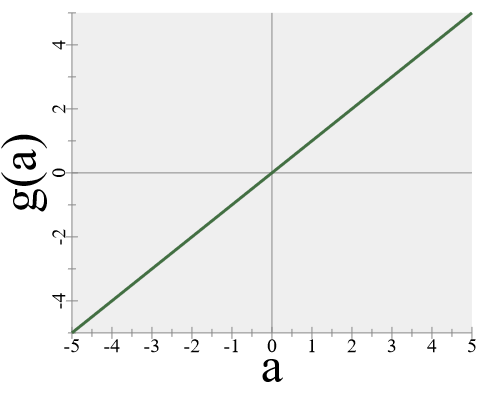
\includegraphics[width=\textwidth]{images/4_linear.png}
        \caption{Linear}
        \label{fig:activation_linear}
    \end{subfigure}
    \begin{subfigure}[b]{0.3\textwidth}
        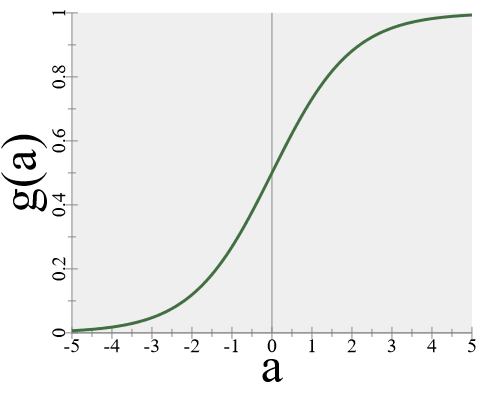
\includegraphics[width=\textwidth]{images/4_sigmoid.png}
        \caption{Logistic sigmoid}
        \label{fig:activation_sigmoid}
    \end{subfigure}
    \begin{subfigure}[b]{0.3\textwidth}
        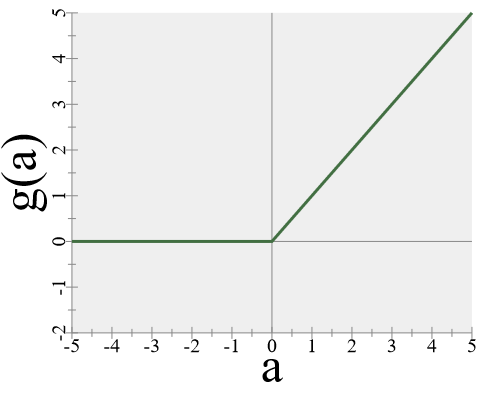
\includegraphics[width=\textwidth]{images/4_relu.png}
        \caption{ReLU}
        \label{fig:activation_relu}
    \end{subfigure}
    \caption{Activation functions}
    \label{fig:activation}
\end{figure}

Mathematical representations are shown in equation~\eqref{eq:sigmoid_relu}

\begin{equation}
    \begin{split}
        Sigmoid: f(x) & = \frac{1}{1 + \exp^{-x}} \\ ReLU: f(x) & = max(0, x)
    \end{split}
    \label{eq:sigmoid_relu}
\end{equation}

The use of the activation functions can also vary; for example, it is common for the logistic sigmoid to have a threshold to not fire at all if a certain value (e.g. 0.5) is not reached.

With the introduction of activation functions, the equations ~\eqref{eq:node_value} and \eqref{eq:node_value_vectorized} become equal:

\begin{equation}
    a^l_j = \sigma(z^l_j) = \sigma(\sum^n_{i=0}z^{l-1}_i\theta^l_{i, j})
    \label{eq:activation}
\end{equation}

With the corresponding vectorized equation:

\begin{equation}
    a^l = \sigma(z^l) = \sigma(\theta^l z^{l-1})
    \label{eq:activation_vectorized}
\end{equation}

There are a variety of different activation functions, these two being the most prominent.
The selection of the activation function and possibly a corresponding threshold value is another hyperparameter that must be selected before the training.

\subsection{Backpropagation}

With gradient descent~\eqref{eq:gradient_descent} not all parameters in all layers can be updated, because it only considers updating the parameters of the last level if it is considered independent of previous layers.
Since the last layer is a function of the previous layer, the chain rule can be applied and thus apply the calculated error of the last layer to the preceding one and update the weights and biases. This applies to every layer, except the input layer (which does not need to be updated in the end).
The following equations are derived using \cite[p.733]{StuartRussell2018}, \cite[p.197]{Goodfellow2017} and \cite[ch.2]{Nielsen2015}:

\begin{equation}
    \varDelta^L = \nabla_a L \odot \sigma'(z^L)
    \label{eq:output_error}
\end{equation}
\begin{equation}
    \varDelta^l = ((\theta^{l+1})^T \varDelta^{l+1}) \odot \sigma'(z^l)
    \label{eq:hidden_error}
\end{equation}
\begin{equation}
    \theta_{i+1} := \theta_i - \eta \varDelta
    \label{eq:backprop_update}
\end{equation}

Equation~\eqref{eq:output_error} describes the error calculated in the output layer. We define our network with $L$ layers, so the output layer is always described by the $L$ index.
$\odot$ is the Hadamard operator. It is used to multiply tensors element by element, which is useful in this case as it prevents the vectors from having to be transformed into diagonal matrices.
Equation~\eqref{eq:output_error} is a direct result of applying the multivariate chain rule to the derivative of the loss function performed in the last layer.
As mentioned above, the gradient descent is performed by the derivative of the loss function in equation~\eqref{eq:sgd_mse_here}.
Since an activation function is implemented between the input used in the loss function and the output of the previous layer, the chain rule must also be applied to the latter.

\begin{equation}
    \frac{\partial L}{\partial z^L_j} = \frac{\partial L}{\partial a^L_j}\frac{\partial a^L_j}{\partial z^L_j}
    \label{eq:proof_loss_chain_rule}
\end{equation}

By pointing out that $\frac{\partial L}{\partial a^L_i}$ is only a non-vectorized form of $\nabla_a L$ and $\frac{\partial a^L_i}{\partial z^L_i}$ of $\sigma'(z^L)$ the equivalence becomes clear.

Equation~\eqref{eq:hidden_error} can be rewritten as follows:

\begin{equation}
    \varDelta^l_i = \frac{\partial L}{\partial z^l_i} = \sum_{j=0}^n (\frac{\partial L}{\partial z^{l+1}_j}\frac{\partial z^{l+1}_j}{\partial z^l_i})
\end{equation}

$n$ is the number of nodes in the next layer. From $\frac{\partial L}{\partial z^{l+1}_i} = \varDelta^{l+1}_i$ follows:

\begin{equation}
    \frac{\partial L}{\partial z^l_i} = \sum_{j=0}^n (\varDelta^{l+1}_j \frac{\partial z^{l+1}_j}{\partial z^{l}_i})
    \label{eq:hidden_error_intermediate}
\end{equation}

The following equation is also known:

\begin{equation}
    \begin{split}
    z^{l+1}_j & = \sum_{i=0}^n \theta^{l+1}_{i,j} a^l_i = \sum_{i=0}^n \theta^{l+1}_{i, j} \sigma(z^l_i) \\
    \frac{\partial z_j^{l+1}}{\partial z_i^l} & = \theta^{l+1}_{i,j} \sigma'(z^l_j)
    \end{split}
\end{equation}

So we can substitute the terms in equation~\eqref{eq:hidden_error_intermediate}:

\begin{equation}
    \frac{\partial L}{\partial z^l_i} = \sum_{j=0}^n (\varDelta^{l+1}_j \theta^{l+1}_{i,j} \sigma'(z_j^l))
\end{equation}

Which again is just a non-vectorized form of the equation ~\eqref{eq:hidden_error}.

Equation~\eqref{eq:hidden_error} is then executed on each layer until $l=0$ is reached and a $\varDelta$ is calculated for each parameter in $\theta$, which are applied by equation~\eqref{eq:backprop_update}.
This type of backward propagation gave this algorithm the prominent name of "backpropagation" (short for "backward propagation of error" \cite{Rumelhart1986}).

\subsection{Generalization}

The task of any algorithm for machine learning is to generalize.
After the model has been trained with data, it should also achieve good results with data it has never seen before.
This distinguishes machine learning from optimization problems (which could be solved with the Newton-Raphson method, for example).

However, a generalization is not guaranteed. In particular the phenomena of over- and underfitting  pose problems.
For example, a model that has been trained for a classification task might make correct predictions for training examples, but not work reliably with new data (overfitting).
This indicates that the model has, so to speak, memorized the training examples.
There are some things which can be done to solve this issue.
Giving the model more data for training is a solution shown by Banko and Brill \cite {Banko2001} and commented by Halevy, Norvig and Pereira in their article "The Unreasonable Effectiveness of Data" \cite{Halevy2009}.
Adding a lot of data is not always possible because generating data can be costly, so some compromises may have to be made to solve this problem.

Another possibility is to reduce the number of features in the training data; apparently unintuitive at first glance, it becomes clear that an abundance of features does not add much information to an image. For example, to recognize a handwritten digit, many more parameters have to be adjusted if a high-resolution image with hundreds of thousands of pixels is fed into the model, where a pixel count of less than a thousand would already be sufficient \cite{Nielsen2015}.

On the other hand, the problem of underfitting is as problematic as overfitting.
If the model is already not getting sufficient results from the training data, the problem is called underfitting.
If this is the case, it is likely that the model or parameter will need to be adjusted, or that the training data is unsuitable for the problem.
Furthermore, for the equations~\eqref{eq:universal_approx} and \eqref{eq:hypothesis} to be true for a reasonable model, a rule of thumb is that mapping the input to the expected output should be at least relatable to a human.

In order to train a model for the recognition of mechanical symbols using these techniques, the corresponding data must first be generated.
